% pessoa@angulosolido.pt
%
\documentclass{llncs}
%
\usepackage{makeidx}  % allows for indexgeneration
\usepackage{graphicx} % allows for image insertion
%
\begin{document}
%
\frontmatter          % for the preliminaries
%
\pagestyle{headings}  % switches on printing of running heads
%
\mainmatter              % start of the contributions
%
\title{Framework for improving operations management}
%
\titlerunning{Improving operations management}  % abbreviated title (for running head)
%                                     also used for the TOC unless
%                                     \toctitle is used
%
\author{Pedro Pessoa}
%
\authorrunning{Pedro Pessoa} % abbreviated author list (for running head)
%
%%%% list of authors for the TOC (use if author list has to be modified)
\tocauthor{Pedro Pessoa}
%
\institute{Universidade de \'Evora, \'Evora, Portugal,\\
\email{pessoa@angulosolido.pt}}

\maketitle              % typeset the title of the contribution

\begin{abstract}
Reliable systems need reliable people to run them. As systems administration density\footnote{Systems administration density may be defined as the ratio between servers, physical or virtual, and services, typically provided by a third party, being configured and administered} and complexity increases, so does the impact of the human administrator decisions and actions. Good decisions are taken not only when the human administrator is aware of their systems current state but also when the human operator themselves are both physically and mentally well. This PhD is aimed at the development of a framework for improving how systems administration is impacted by the human component of the systems and which tool set can be provided to better support them.
\keywords{systems administration, operations, sysadmin, devops, humanops, burnout, monitoring}
\end{abstract}
%
\section{Introduction}
%
Human administrators are a fundamental part of any modern computerized systems. They are not only interacting with the systems when failures occur but also when introducing requested changes to running systems. Personality characteristics of these administrators have a direct influence on the reliability of this systems as well as their daily physical and mental state.

"You are not immutable. You are not highly available. You are ephemeral"\footnote{https://www.devopsdays.org/events/2016-london/program/oliver-wood/}.

"People are more difficult to work with than machines. And when you break a person, he can't be fixed".\cite{ric:rio}

An important part of systems administration work is bound to anomaly and pattern recognition, such as when diagnosing a misbehaving cluster member during an incident - figure \ref{fig:Screenshot_20170304_155530.png} - or predicting growth - figure \ref{fig:Screenshot_20170307_134821.png}. That capacity is expected to be always available, in any mindset. Automating this will allow to run more reliable systems by guaranteeing that, in any circumstances, the results will be comparable, thus shifting the responsibility to make those recognitions from the human administrator.

\begin{figure}
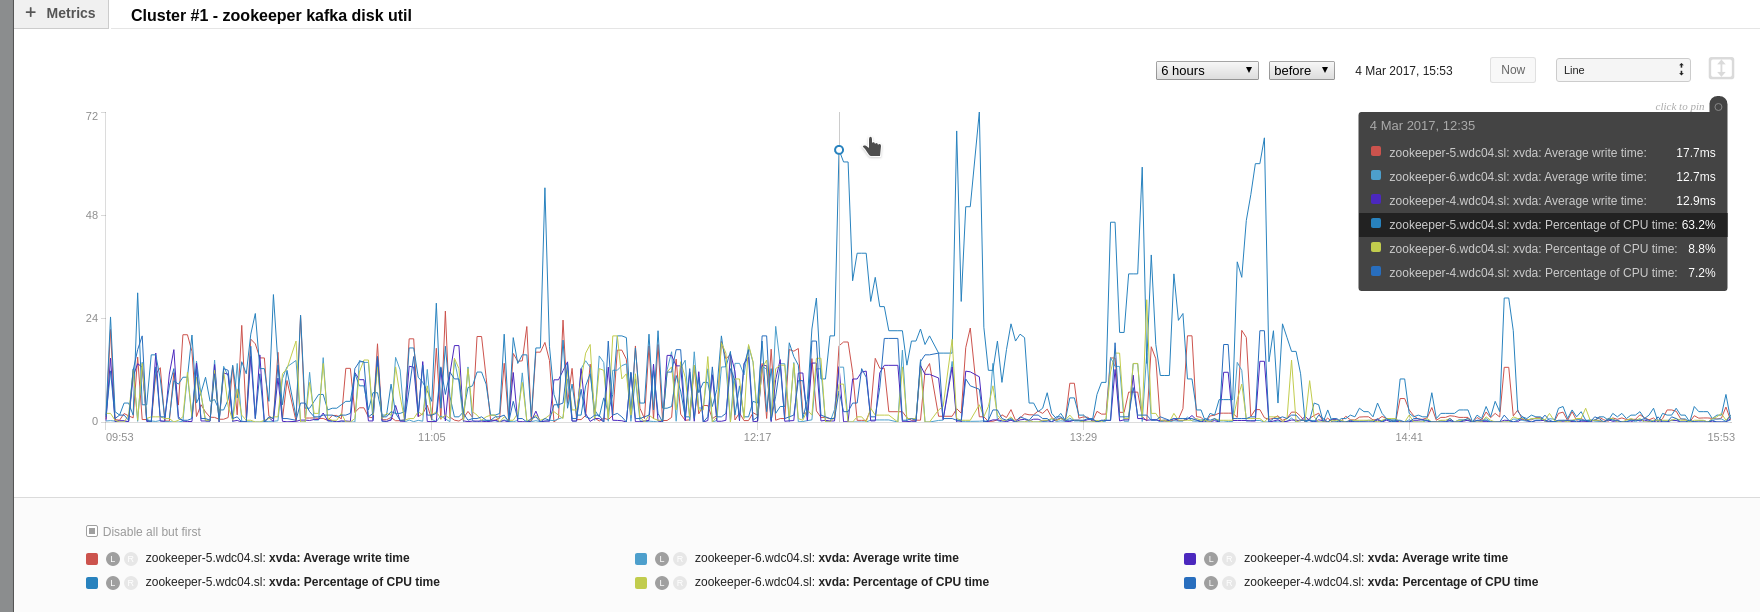
\includegraphics[width=\linewidth]{images/Screenshot_20170304_155530.png}
\caption{Identifying a misbehaving cluster member}
\label{fig:Screenshot_20170304_155530.png}
\end{figure}

\begin{figure}
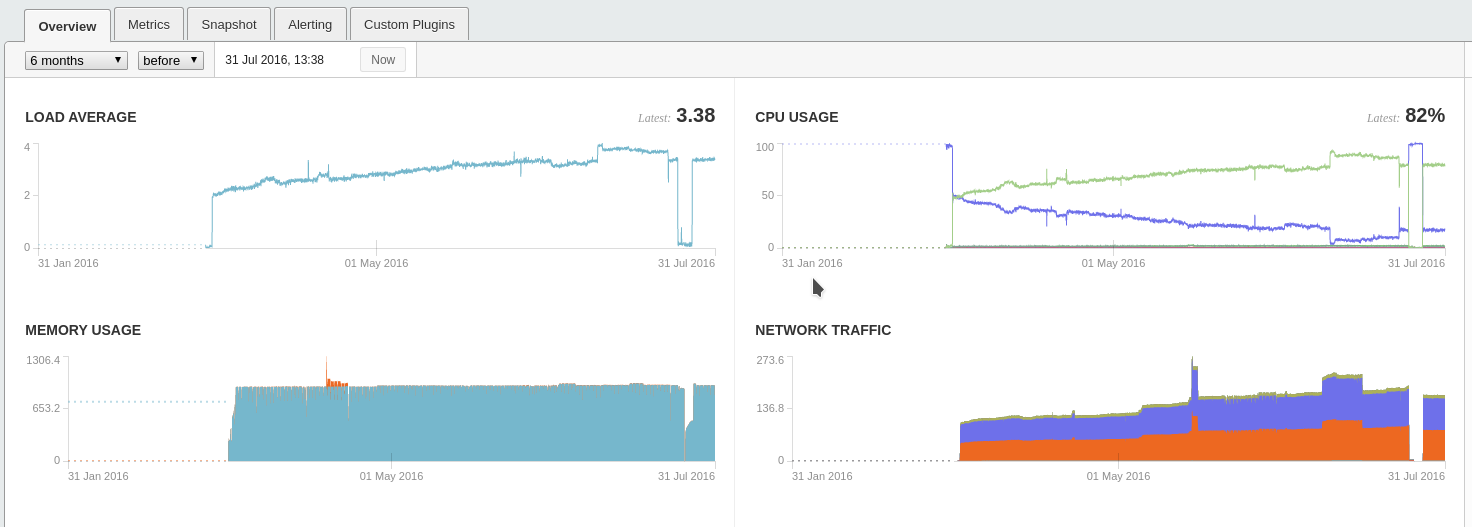
\includegraphics[width=\linewidth]{images/Screenshot_20170307_134821.png}
\caption{Usage growth}
\label{fig:Screenshot_20170307_134821.png}
\end{figure}

This PhD will survey practices such as people profiling for demanding tasks, stress management or burn out prevention as well as the state of the art on pattern identification and machine learning  with the goal to improve or develop recruiting processes, on-call scheduling and monitoring and alerting methodologies resulting in better human systems administrators work output.
%
\section{Prior Work}
%
\subsection{Psychological}
%
"Resilience is not a trait that people either have or don’t have. It involves behaviors, thoughts, and actions that can be learned and developed in everyone.\footnote{http://www.apa.org/helpcenter/road-resilience.aspx}"

Some IT professionals make better systems administrators than others. However it is not well understood what contributes to those differences, or if those differences can be reduced by training or if they are tied in with individual personality characteristics.
%
\subsection{Tools}
%
Having tools and devices available to track well being, healthy or sleep patterns, will allow to correlate those to alerts from the systems being administered.

Some examples follow.

An activity tracker device such as the Fitbit\footnote{https://www.fitbit.com/eu/shop/flex2} allows to monitor sleep patterns. These can then be correlated to paging alerts from an on-call rotation. Such an application is Opzz\footnote{https://opzzz.sh}

The previous examples can be used to enhance current commercial offers such as an alert cost calculator\footnote{https://blog.serverdensity.com/introducing-alert-costs/}. From a simplistic calculation such as:
\begin{equation}
TEO + (NE * 23)
\end{equation}
showing interruption cost\footnote{http://www.fastcompany.com/944128/worker-interrupted-cost-task-switching} when TEO is the total time an event is open and NE is the number of such events. Such enhancements will feed additional human impact costs and allow developing of an on-call rotation model.

Building on the prior work on intrusion detection \cite{ped:sal}, by using constrains for detection of events that span multiple devices or time will allow to correlate events that will support either systems corrective actions or alert configuration suggestion.
%
\section{High Level Planning}
%
At present, this PhD is surveying the psychological aspects and studies applicable to operations and systems administration. This should tie in with selecting and improving automation of tasks likely to be executed by systems administrators, during stressful periods, by matching to mined device alerting data.

Having access to approximately 7TiB of raw metrics data from 700.000 devices, 74.000 alert configurations manually made by 20.000 anonymized users will allow verification of the automation models to be developed.
%
\section{Conclusion}
%
By accepting that systems will always require human intervention for operations that cannot be automated, and by recognizing and predicting the weakest aspects of the human operator, the goal of this PhD is to contribute on improving automations and failsafe, effectively making the systems administrator job easier in delivering more reliable systems: "operate at a high level of abstraction, relying upon lots of backup systems as failsafes and thoughtful APIs to communicate with the systems."\cite{bet:mur}
%
% ---- Bibliography ----
%
\begin{thebibliography}{5}
%
\bibitem {bet:mur}
Betsy Beyer, Jennifer Petoff, Chris Jones, Niall Richard Murphy:
Site Reliability Engineering: How Google Runs Production Systems.
O′Reilly; 1 edition (8 April 2016).
ISBN-13: 978-1491929124.

\bibitem {ric:rio}
Rick Riordan:
The Battle of the Labyrinth (Percy Jackson and the Olympians, Book 4).
Disney-Hyperion; Reprint edition (April 7, 2009).
ISBN-13: 978-1423101499.

\bibitem {ped:sal}
Pedro Salgueiro, Daniel Diaz, Isabel Brito, and Salvador Abreu:
Using Constraints for Intrusion Detection: the NeMODe System.
In Ricardo Rocha and John Launchbury, editors, PADL’11 - Thirteenth International Symposium on Practical Aspects of Declarative Languages, volume 6539 of Lecture Notes in Computer
Science, pages 115–129, Berlin, Heidelberg, January 2011. Springer-Verlag.
ISBN 978-3642183775.

\end{thebibliography}

\clearpage
\end{document}
